\documentclass{article}
\usepackage[utf8]{inputenc}

\title{NTIN066 - Splay tree}
\author{Thuong-Hai Pham}
\date{October 2017}

\usepackage{graphicx}

\begin{document}

\maketitle

\section{Uniform subset test} \label{uni}

\begin{figure}[ht]
\centering
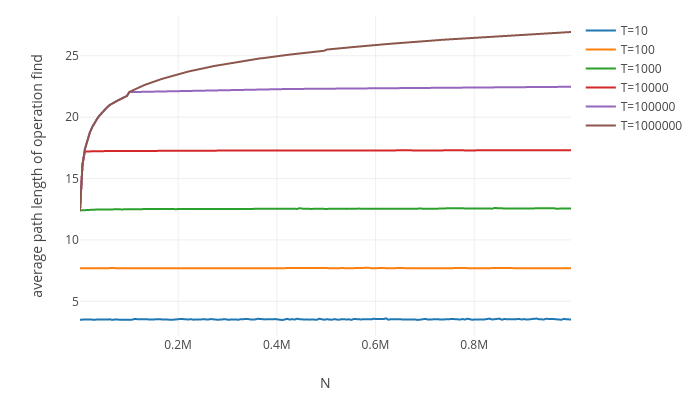
\includegraphics[width=\textwidth]{NTIN066-plot1.png}
\caption{Classical Splay tree and uniform subset test}
\label{fig:plot1}
\end{figure}

Figure \ref{fig:plot1} shows that the curve $T=1000000$ obviously illustrate the complexity is $O(\log(N))$.

However, $T=100000$ follows the curve $O(\log(N))$ for $N\le100000=T$, then turns to a nearly flat line. This phenomenon happens because when $N\le T$, the depth of the tree is $O(\log(N))$. In contrary, when $N>T$, for a randomly chosen value $a$, the first splay operation that brings $a$ to the root costs $O(\log(N))$, the rest 999 slay operation to find $a$ only concerns the sub-tree of depth $O(\log(T))$ from the root (at most T-1 other nodes have been splayed). Hence, the complexity from this point onward is $O(\log(T))$ instead, with T is a constant for each line in Figure \ref{fig:plot1}.

The same explanation applies for $T=10000$, while with $T\le 1000$, there is no $N$ that $N<T$, so they display nearly flat lines from the first data point.

\begin{figure}[h!]
\centering
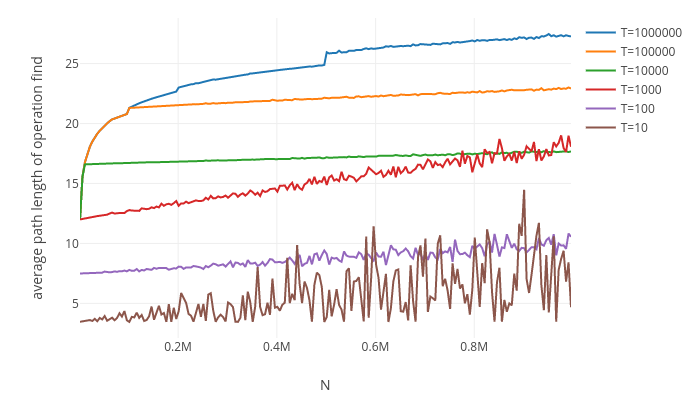
\includegraphics[width=\textwidth]{NTIN066-plot2.png}
\caption{Naive Splay tree and uniform subset test}
\label{fig:plot2}
\end{figure}

\begin{figure}[h!]
\centering
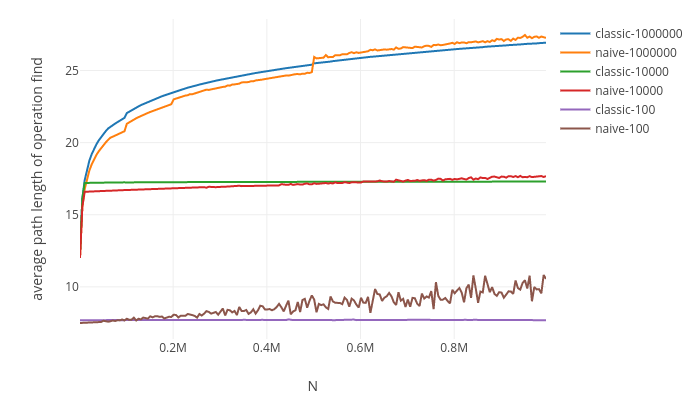
\includegraphics[width=\textwidth]{NTIN066-plot3.png}
\caption{Classical and Naive Splay tree with uniform subset test}
\label{fig:plot3}
\end{figure}

Figure \ref{fig:plot2} shows result from the same test set, yet with Naive Splay tree. It is clear that the phenomenon of $N>T$ still exists. In addition, the average path length of operation find for small $T \in \{10,100,1000\}$ fluctuates and has higher value when increasing $N$.

Figure \ref{fig:plot3} illustrates this point by comparing between the Classical and Naive Splay tree. This is due to the fact that Naive Splay tree does not guarantee to maintain a balanced search tree in worst cases which one of them will be discussed further in Section \ref{seq}.

\section{Sequential test} \label{seq}

Figure \ref{fig:plot4} exhibits the difference in performance (average path length of operation find) between Classical and Naive Splay tree with sequential test. In this type of test set, the generator generates a sequence of operations to insert each integer from $1$ to $N$, then a sequence of operations to find an integer from $1$ to $\frac{N}{2}$, in that order, then repeats this find sequence again.

While Classical Splay tree complexity is $O(\log(N))$ (Figure \ref{fig:plot4}, \ref{fig:plot4a}), Naive Splay tree performs worse with a complexity of $O(N)$.

\begin{figure}[h!]
\centering
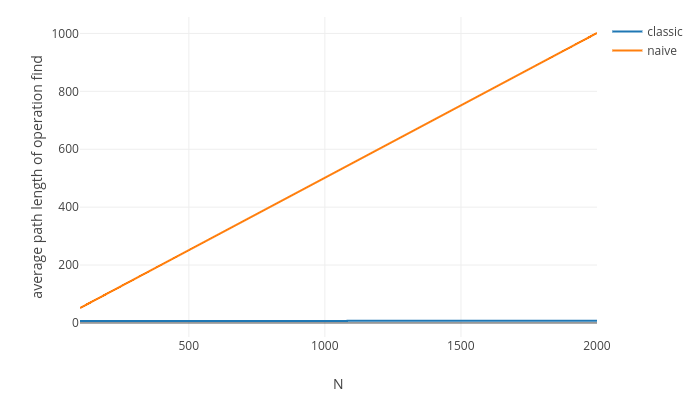
\includegraphics[width=\textwidth]{NTIN066-plot4.png}
\caption{Classical and Naive Splay tree with sequential test}
\label{fig:plot4}
\end{figure}
\begin{figure}[h!]
\centering
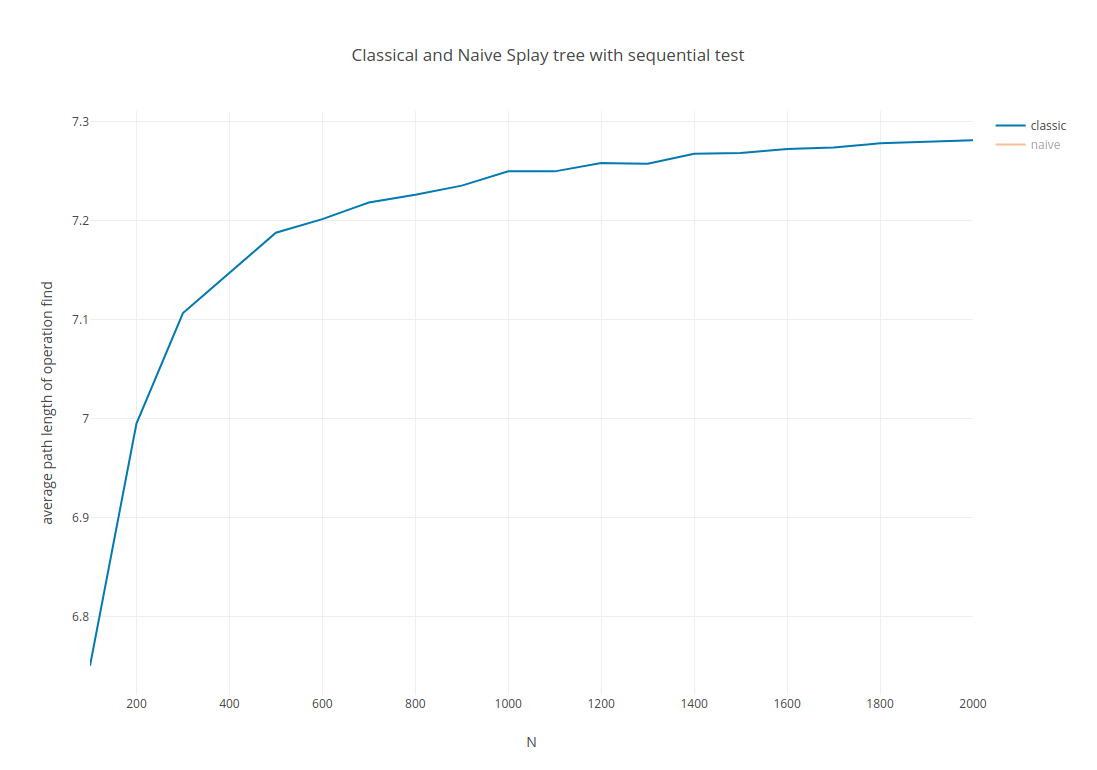
\includegraphics[width=\textwidth]{NTIN066-plot4a.png}
\caption{Classical tree with sequential test}
\label{fig:plot4a}
\end{figure}
\begin{figure}[h!]
\centering
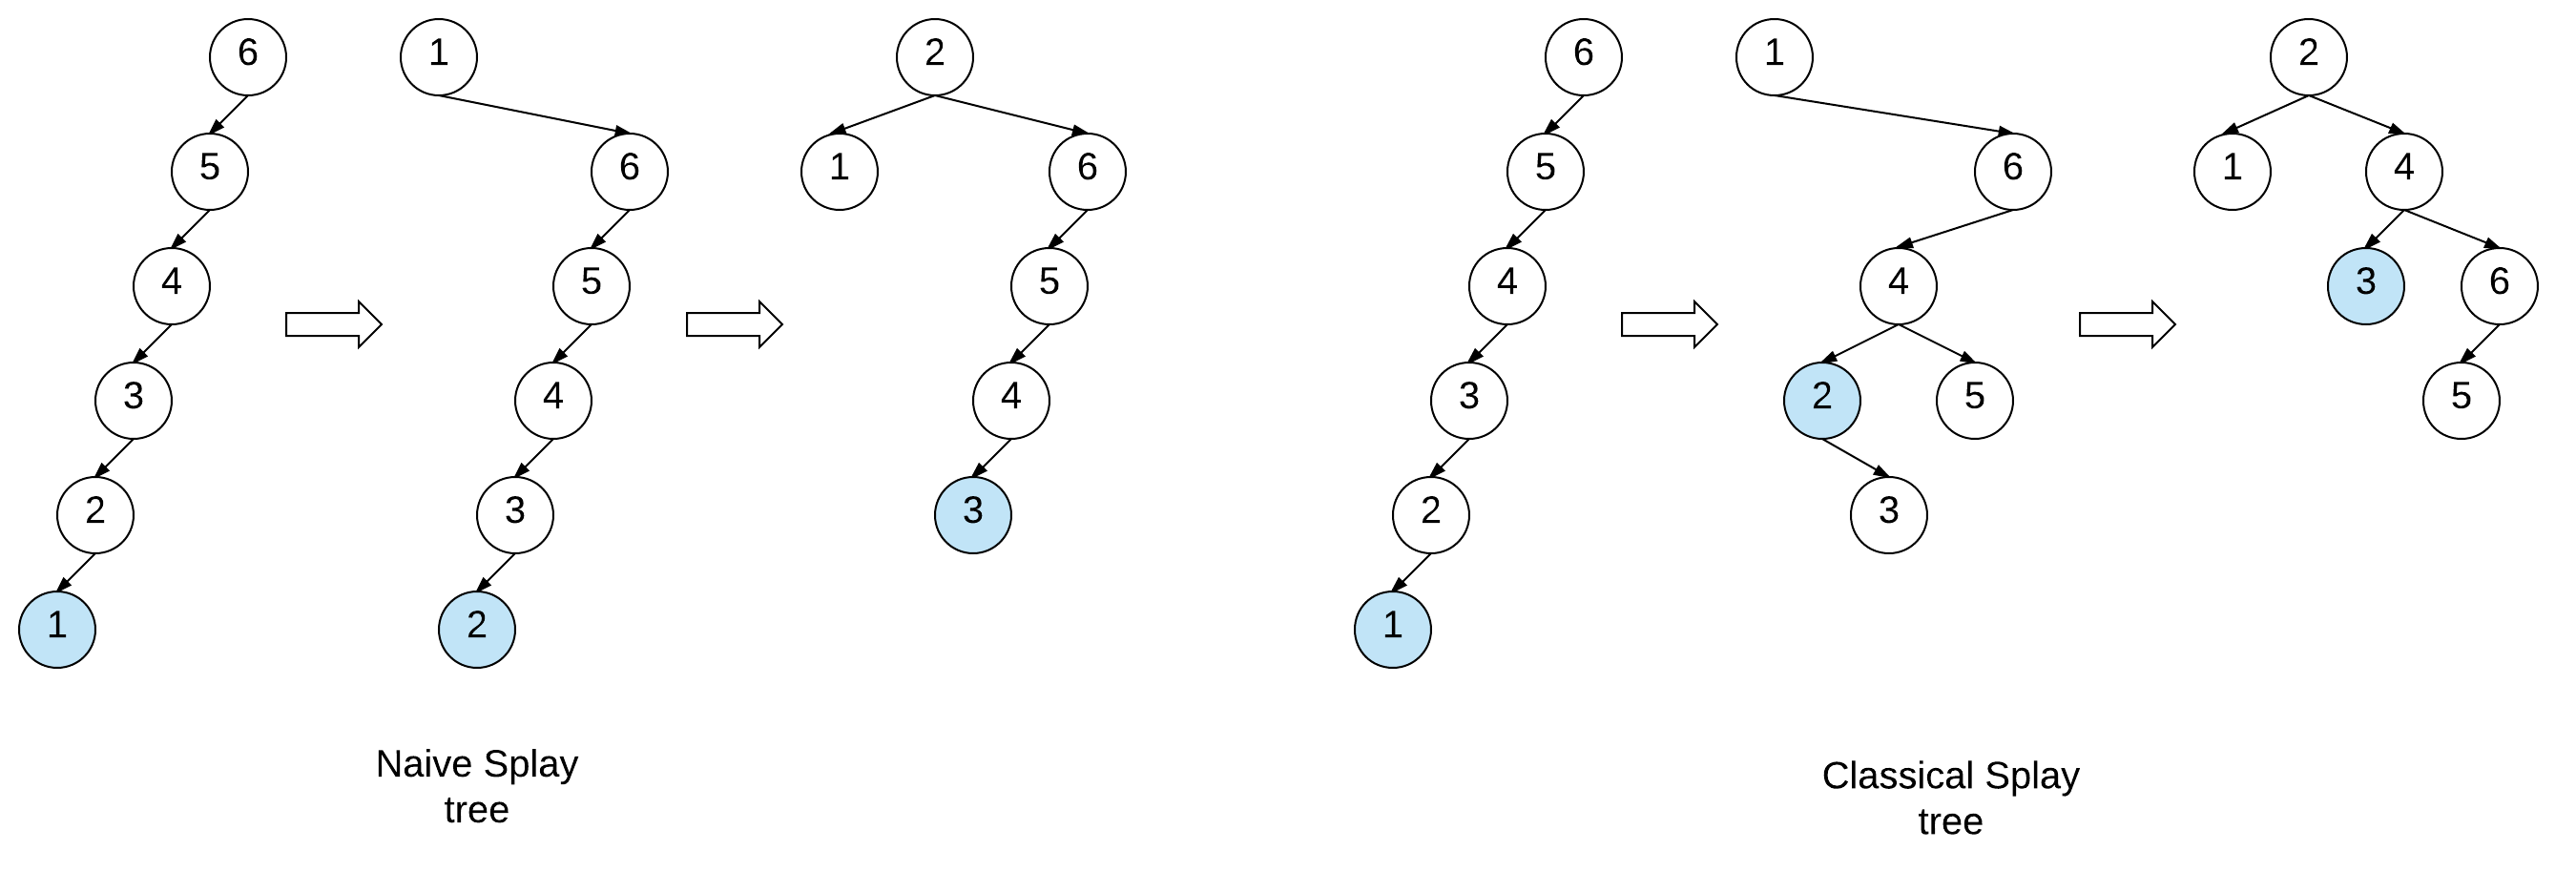
\includegraphics[width=\textwidth]{naive-seq.png}
\caption{Naive and Classical Splay tree with N=6 in sequential test}
\label{fig:naive-seq}
\end{figure}

To study the reason, let us take a trivial example of $N=6$. Figure \ref{fig:naive-seq} demonstrates the first tree find operations on both Naive and Classical Splay tree for $N=6$. In this example, Classical Splay tree, when performing splay operation for a node, reduces the path length of that node's ancestor down to half. Hence, after a small number of find operations, the tree will reduces its depth to $O(\log(N))$.

On the other hand, Naive Splay tree keeps the long array-like tree when it splays. Therefore, node with value ``1" (node ``1") to find has the depth of $N$, the same for node ``2". From node $i=$``3" onward, its depth is $N-i+2$, because $i-2$ nodes have been moved to the left subtree of the root. With that observation, the total depth of nodes that values are to find in the first ``find" sequence is $$D_1=N+\sum_{i=2}^{N/2}(N-i+2)=\sum_{i=1}^{N/2}(N-i+2)-1=\frac{3N^2}{8}+\frac{3N}{4}-1$$

The same formula can be applied for the second ``find" sequence with the observation that after the first ``find" sequence, the right subtree will be discarded (node with value $>\frac{N}{2}$). Hence, we can consider a new tree of depth $N'=\frac{N}{2}$ that has the same structure with our original tree before all ``splay" operation. Consequently, the total depth for this second ``find" sequence is
$$D_2=\sum_{i=1}^{N'/2}(N'-i+2)-1=\sum_{i=1}^{N/4}\left(\frac{N}{2}-i+2\right)-1=\frac{N^2}{8}+\frac{3N}{4}-1$$
and the average path length of this Naive Splay tree is
$$\frac{D_1+D_2}{N}=\frac{N}{2}+\frac{3}{2}-\frac{2}{N}$$

which is also the exact formula of ``naive" line in Figure \ref{fig:plot4} and explains the complexity of $O(N)$.


\subsection*{Effect of -l parameter}

With ``-l" parameter, the generator instead samples values for ``F" command from the whole arrays, now only considers the $T$ recently inserted values (the last $T$ elements of insertion sequence). Hence, in this case, splay operations merely need to deal with a smaller subtree from the root of the tree, which includes recently inserted nodes. This is shown in Figure \ref{fig:plot6}, which clearly favors the case of smaller $T$ in compare to $N$. Therefore, the comparison between Classical and Naive splay tree with uniform subset test should be conducted without ``-l" parameter as we did in Section \ref{uni}.

\begin{figure}[h!]
\centering
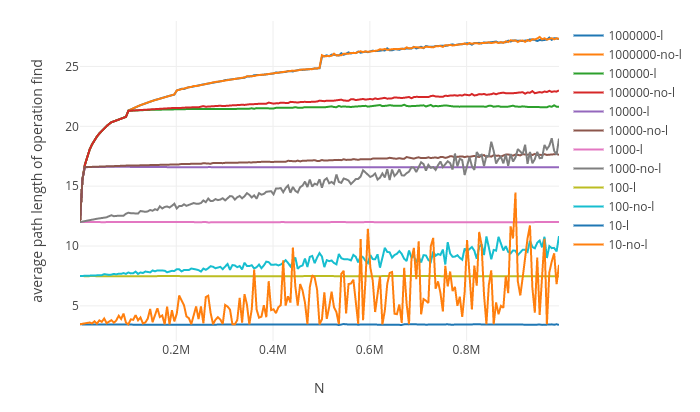
\includegraphics[width=\textwidth]{NTIN066-plot6.png}
\caption{Naive Splay tree with different sampling methods for uniform subset test}
\label{fig:plot6}
\end{figure}

\end{document}
